[95 r\textsuperscript{o}] \edtext{Cur}{\lemma{patet.}\Afootnote{ \textit{ (1) }\ Ex his  \textbar\ nihil puto \textit{ gestr.}\ \textbar\  ratione principali phaenomenon manifestius \textit{ (2) }\  Cur \textit{ L}}} \edtext{Tabulae duae bene politae}{\lemma{Cur}\Afootnote{ \textit{ (1) }\ Laminae\protect\index{Sachverzeichnis}{laminae politae|textit} \textit{ (2) }\ Tabulae duae   \textbar\ bene politae \textit{ erg.}\ \textbar\  \textit{ L}}} in Recipiente quoque exhausto ubi nulla 
% \begin{wrapfigure}{l}{0.4\textwidth}                    
    %            
\includegraphics[width=0.4\textwidth]{images/37_3_95r1}
        %         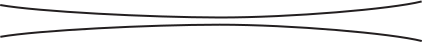
\includegraphics[width=0.4\textwidth]{images/37_3_95r2}
                        %\caption{Bildbeschreibung}
            %            \end{wrapfigure} 
            est aeris \edtext{pressio\protect\index{Sachverzeichnis}{pressio!aeris}, a pondere appenso non divellantur ex iisdem causis  facile intelligitur}{\lemma{pressio,}\Afootnote{ \textit{ (1) }\ continuantur \textit{ (2) }\ ex his facile intelli \textit{ (3) }\ a [...] intelligitur \textit{ L}}}; non possunt enim a se invicem \edtext{divelli}{\lemma{invicem}\Afootnote{ \textit{ (1) }\ separari \textit{ (2) }\ divelli \textit{ L}}}, quin  primo ut sic dicam momento \edtext{divulsionis}{\lemma{momento}\Afootnote{ \textit{ (1) }\ dissolutionis \textit{ (2) }\ divulsionis \textit{ L}}} locus \edtext{relinquatur materia}{\lemma{relinquatur}\Afootnote{ \textit{ (1) }\ aere \textit{ (2) }\ materia \textit{ L}}} circumfusa vacuus, quae subire satis cito, non potest, \edtext{si}{\lemma{potest,}\Afootnote{ \textit{ (1) }\ nam \textit{ (2) }\ cum \textit{ (3) }\ si \textit{ L}}} primo statim momento divellantur \edtext{ubique,}{\lemma{divellantur}\Afootnote{ \textit{ (1) }\ omnino \textit{ (2) }\ ubique,  \textbar\ quo casu \textit{ gestr.}\ \textbar\  \textit{ L}}} necesse esset enim  aerem \edtext{circumfusum}{\lemma{aerem}\Afootnote{ \textit{ (1) }\ diffusum \textit{ (2) }\ circumfusum \textit{ L}}} momento ad mediam usque laminam  pervenire, quod impossibile est, aut \edtext{laminam avellendam.  Ut ergo divelli queant, necesse est incurvari}{\lemma{aut}\Afootnote{ \textit{ (1) }\ laminas\protect\index{Sachverzeichnis}{laminae politae|textit} incurvari, duas ut citius \textit{ (2) }\ laminam [...] incurvari \textit{ L}}} in \edtext{superficiem curvam,  quae convexitatem alteri obvertat}{\lemma{in}\Afootnote{ \textit{ (1) }\ duas superficies curvas convexitatem  sibi obvertentes \textit{ (2) }\ superficiem [...] obvertat \textit{ L}}}, 
   %@ @ @ Dies ist eine Abstandszeile - fuer den Fall, dass mehrere figures hintereinander kommen, ohne dass dazwischen laengerer Text steht. Dies kann zu einer Fahlermeldung fuehren. @ @ @ \\
                    %  \begin{wrapfigure}{l}{0.4\textwidth}                    
                %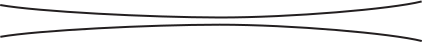
\includegraphics[width=0.4\textwidth]{images/37_3_95r2}
                        %\caption{Bildbeschreibung}
                    %    \end{wrapfigure}
                        %@ @ @ Dies ist eine Abstandszeile - fuer den Fall, dass mehrere figures hintereinander kommen, ohne dass dazwischen laengerer Text steht. Dies kann zu einer Fahlermeldung fuehren. @ @ @ \\
                     ac proinde prius in extremis quam \edtext{medio, ab ea abeat,}{\lemma{medio,}\Afootnote{ \textit{ (1) }\ a se  abire, aut \textit{ (2) }\ ab ea abeat, aut \textit{ L}}} \edtext{aut necesse est}{\lemma{aut}\Afootnote{ \textit{ (1) }\ quod \textit{ (2) }\ quae laminarum\protect\index{Sachverzeichnis}{laminae politae|textit} incurvatio difficilis, aut denique \textit{ (3) }\  necesse est \textit{ L}}} \edtext{ex}{\lemma{est}\Afootnote{ \textit{ (1) }\ aere in \textit{ (2) }\ ex \textit{ L}}} materia circumfusa exprimi aliam \edtext{ad penetrandos Tabulae}{\lemma{aliam}\Afootnote{ \textit{ (1) }\ subtiliorem ad penetrandam laminam \textit{ (2) }\ ad penetrandos  \textit{(a)}\ laminae\protect\index{Sachverzeichnis}{laminae politae|textit} \textit{(b)}\ Tabulae \textit{ L}}} poros satis  subtilem. Utrumque non sine viribus satis magnis fieri  potest.\pend 
%                      %       \begin{wrapfigure}{l}{0.4\textwidth}                    
%                \begin{center}
%                 
\includegraphics[width=0.4\textwidth]{images/37_3_95r1}
%                 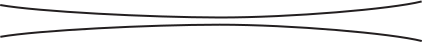
\includegraphics[width=0.4\textwidth]{images/37_3_95r2}\\\textit{[Fig. 2]}\protect\rule[0cm]{4cm}{0cm}\textit{[Fig. 3]}\\
%                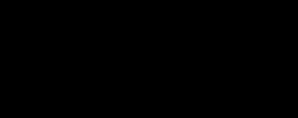
\includegraphics[width=0.4\textwidth]{images/37_3_95r3}\\\textit{[Fig. 4]}
%                        %\caption{Bildbeschreibung}
%                    %    \end{wrapfigure}
%                    \end{center}
                     \pstart  Ut haec jam determinentur sequentia \edtext{experimenta}{\lemma{}\Afootnote{experimenta \textit{ erg.} \textit{ L}}} institui possunt: experiendum  est faciliusne tabulae\protect\index{Sachverzeichnis}{tabulae!politae} divellantur, si pondus\protect\index{Sachverzeichnis}{pondus} extremis, an  si medio inferioris sit appensum, nam si extremis appensum citius  divellit, signum est superficies fuisse incurvatas. \edtext{Item an difficilius divellantur si extrema Tabularum\protect\index{Sachverzeichnis}{tabulae!politae} ferro ita munita sint, ut difficilius queant incurvari.}{\lemma{Item [...] incurvari.}\Afootnote{\textit{ erg.} \textit{ L}}} Experiendum  est minoribusne viribus in aere exhausto quam libero ordinariove  opus sit; nam si ita, signum est materiam circumfusam  attenuatam per laminae\protect\index{Sachverzeichnis}{laminae politae} poros transire, minoribus enim viribus  opus fuit, ad materiam jam attenuatam amplius attenuandam.  Experiendum est qualis sit materia illa \edtext{si qua est}{\lemma{}\Afootnote{si qua est \textit{ erg.} \textit{ L}}} Tabulis\protect\index{Sachverzeichnis}{tabulae!politae}  momento divulsionis interfusa, \edtext{nam si per  poros laminae transiit, necesse est longe esse materia  illa in Recipientibus exhaustis residua esse subtiliorem.}{\lemma{interfusa,}\Afootnote{ \textit{ (1) }\ sitne  \textit{(a)}\ aere \textit{(b)}\ materia in  recipiente exhausto residua subtilior, q \textit{ (2) }\ nam [...] subtiliorem. \textit{ L}}} Hoc experimentum ita facere licebit. Tabulae\protect\index{Sachverzeichnis}{tabulae!politae} duae  sibi communi more imponantur, 
               %       \begin{wrapfigure}{l}{0.4\textwidth}                    
                %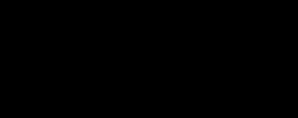
\includegraphics[width=0.4\textwidth]{images/37_3_95r3}
                        %\caption{Bildbeschreibung}
                    %    \end{wrapfigure}
                        %@ @ @ Dies ist eine Abstandszeile - fuer den Fall, dass mehrere figures hintereinander kommen, ohne dass dazwischen laengerer Text steht. Dies kann zu einer Fahlermeldung fuehren. @ @ @ \\
                     \edtext{Tabula una}{\lemma{imponantur,}\Afootnote{ \textit{ (1) }\ extremum unius \textit{ (2) }\  quaelibet extremo unius \textit{ (3) }\ Tabula  \textit{(a)}\ quaelibet \textit{(b)}\ una \textit{ L}}} circumdetur crena  profunde excavata in quam eminentia alterius  exacte intret; ut commissura sit justior \edtext{caementum illinatur quale aeri excludendo adhibitum est, ita tabulis}{\lemma{caementum}\Afootnote{ \textit{ (1) }\ illis \textit{ (2) }\ illinatur [...] tabulis \textit{ L}}}  per vim tandem diductis aer externus intrare non poterit.  Ergo aut Tabulae\protect\index{Sachverzeichnis}{tabulae!politae} nunquam sic diducentur, sed potius  omnia rumpentur, quod signum erit ad laminas\protect\index{Sachverzeichnis}{laminae politae} divellendas  opus esse marginum incurvatura; aut si diducentur, materia  intus replebitur spatium, omni illa quam hactenus assecuti  sumus subtiliore. \edtext{Quae scilicet per caementi laminarumve poros pervaserit; in qua}{\lemma{subtiliore.}\Afootnote{ \textit{ (1) }\ Et si \textit{ (2) }\ Poterit \textit{ (3) }\   \textbar\ Quae [...] pervaserit; \textit{ erg.}\ \textbar\  in qua \textit{ L}}} novus experimentorum  campus aperietur. \edtext{Poterit enim in eam Epistomio\protect\index{Sachverzeichnis}{epistomium} admitti aer externus, poterit ipsa exhauriri amplius, pot\-erunt foramina ad inspiciendum aperiri, poterunt animalia immitti.}{\lemma{Poterit [...] poterunt}\Afootnote{\textit{ (1) }\ corpora immitti \textit{ (2) }\ animalia immitti. \textit{ erg.} \textit{ L}}} Manifestum est hoc experimentum  fieri posse si Tabulae\protect\index{Sachverzeichnis}{tabulae!politae} non sint adeo exacte politae, modo illitus liquor\protect\index{Sachverzeichnis}{liquor!purgatus} aliquis aere purgatus \edtext{hiatus expleat}{\lemma{purgatus}\Afootnote{ \textit{ (1) }\ concavitates impleat \textit{ (2) }\ hiatus expleat \textit{ L}}}.  Si pondera ad distrahendum non sufficiunt, poterit cochlea\protect\index{Sachverzeichnis}{cochlea} adhiberi.  Imo sine omni illo apparatu suffecerit embolum\protect\index{Sachverzeichnis}{embolus}  quendam exacte adaptatum esse Tubo, quod caemento illito  faciendum est; ita nihil aeris  inerit. Embolo\protect\index{Sachverzeichnis}{embolus} ergo \edtext{maxima vi}{\lemma{}\Afootnote{maxima vi \textit{ erg.} \textit{ L}}} extracto, necesse est materiam, quae intus \edtext{spatium implet}{\lemma{intus}\Afootnote{ \textit{ (1) }\ est \textit{ (2) }\ spatium implet \textit{ L}}} aut ex ipsis Tubi embolive\protect\index{Sachverzeichnis}{embolus} lateribus caementove fuisse  secretam, aut per eorum poros penetrasse. Hac methodo  poterit vas aliquod omni penitus aere evacuari, cum in  Recipiente exhausto possibile sit superesse aerem summe  dilatatum. \edtext{Et in hac materia tam subtili rursus experiendum erit, faciliusne quam in recipiente exhausto laminae\protect\index{Sachverzeichnis}{laminae politae} aliae divellantur. Poterit enim Tubo inseri fenestella, poterit Tubus ipse vitreus esse si modo non magis hic, quam in communi aeris exhausti experimento, rumpitur.}{\lemma{Et [...] Tubus}\Afootnote{\textit{ (1) }\ ille \textit{ (2) }\ ipse vitreus [...] rumpitur. \textit{ erg.} \textit{ L}}}\pend \pstart  Experimentum etiam sumendum  est an \edtext{eadem vi}{\lemma{an}\Afootnote{ \textit{ (1) }\ majore vi \textit{ (2) }\ eadem vi \textit{ L}}} opus sit ad corpora congruentia  sine aeris ingressu divellenda, et ad Mercurium\protect\index{Sachverzeichnis}{mercurius!purgatus} \edtext{aliumve liquorem\protect\index{Sachverzeichnis}{liquor!purgatus} aere}{\lemma{aliumve}\Afootnote{liquorem\protect\index{Sachverzeichnis}{liquor!purgatus} aere \textit{ erg.} \textit{ L}}} purgatum  a summitate Tubi avellendum. Hoc experiri licebit, si pondus\protect\index{Sachverzeichnis}{pondus} embolo\protect\index{Sachverzeichnis}{embolus} extrahendo appensum; et gravitas\protect\index{Sachverzeichnis}{gravitas} Mercurii\protect\index{Sachverzeichnis}{mercurius} quae  scilicet amplius suspendi negat comparentur, posita scilicet  eadem \edtext{ tubi crassitie utrobique}{\lemma{eadem}\Afootnote{ \textit{ (1) }\ ubique \textit{ (2) }\  tubi crassitie utrobique \textit{ L}}}. Si eadem \edtext{circiter gravitas}{\lemma{circiter}\Afootnote{ \textit{ (1) }\ vis \textit{ (2) }\  gravitas \textit{ L}}}  est,\edtext{}{\lemma{}\Afootnote{est,  \textbar\ tanto magis \textit{ gestr.}\ \textbar\ confirmabitur, \textit{ L}}} confirmabitur, eandem utrobique esse causam.  Experimenta denique sumenda sunt per omne tum corporum solidorum\protect\index{Sachverzeichnis}{corpus!solidum}, tum liquorum genus, \edtext{ut determinentur; corpora}{\lemma{ut}\Afootnote{ \textit{ (1) }\ experimentis  determinemur \textit{ (2) }\  determinentur; corpora \textit{ L}}} quae citius \edtext{avellantur}{\lemma{citius}\Afootnote{ \textit{ (1) }\ divellantur, aut \textit{ (2) }\ avellantur \textit{ L}}}, quae proinde 